
%----------------------------------------------------------------------------------------
%	PREAMBUŁA
%----------------------------------------------------------------------------------------

\documentclass[12pt]{article}
\usepackage[polish]{babel}
\usepackage{polski}
\usepackage[utf8]{inputenc}
%\usepackage[T1]{fontenc}
\usepackage{amsmath}
\usepackage{graphicx}
\usepackage{fancyhdr}
\usepackage{float}
\usepackage{graphicx}
\usepackage{hyperref}
\usepackage{verbatim}

\usepackage{subfig}

\usepackage{color} %red, green, blue, yellow, cyan, magenta, black, white
\definecolor{mygreen}{RGB}{28,172,0} % color values Red, Green, Blue
\definecolor{mylilas}{RGB}{170,55,241}


\title{Sprawozdanie}
\author{Aleksandra Poręba}

\graphicspath{{static/}} 

\makeatletter
\let\thetitle\@title
\let\theauthor\@author
\let\thedate\@date
\makeatother


%----------------------------------------------------------------------------------------
%	STRONA TYTUŁOWA
%----------------------------------------------------------------------------------------
\begin{document}
\begin{center}
\textsc{\normalsize Wydział Fizyki i Informatyki Stosowanej}\\[2.0cm] 

\includegraphics[scale = 1]{logo.png}\\[1cm] 
%\textsc{\Large Modelowanie Procesów Fizycznych}\\[0.4cm] 


\textsc{\Large Sprawozdanie}\\[0.4cm]
{ \huge \bfseries \LARGE{Projekt 1: Gra w życie} }\\[1cm] 

\flushright \Large Aleksandra Poręba \\ nr. indeksu 290514

\vfill 

\center{\today}


\pagebreak 

\end{center}

%----------------------------------------------------------------------------------------
%	SPIS TREŚCI
%----------------------------------------------------------------------------------------
%\tableofcontents
%\pagebreak

%----------------------------------------------------------------------------------------
%	ZAWARTOŚĆ
%----------------------------------------------------------------------------------------

\pagestyle{fancy}
\fancyhf{}

\rhead{\theauthor}
\lhead{\thetitle}
\cfoot{\thepage}

\section{Opis projektu}
W ramach projektu została stworzona aplikacja webowa, prezentująca automat komórkowy, jakim jest gra w życie.

Automatami komórkowymi nazywamy systemy składające się z ułożonych obok siebie komórek. W tym projekcie rozważamy komórki ułożone na płaszczyźnie 2D, stykające się ze sobą bokami. Każda komórka ma więc swoich ośmiu sąsiadów ( otoczenie Moore'a o promieniu 1 ). Prezentowane automaty są binarne, co oznacza, że mają dwa stany: żywa lub martwa.

Przy ustalaniu nowego stanu komórek w kolejnych krokach czasowych, brane są pod uwagę reguły automatu, przedstawione jako parametry STAY / BORN. Oznaczają one ilość żywych sąsiadów, aby komórka \textbf{pozostała} żywa oraz ilość żywych sąsiadów, aby komórka \textbf{stała się} żywa.

Choć teoretycznie plansza z komórkami powinna być nieskończona, niestety nie jest możliwe zaimplementowanie takowej. Siatka w symulacji ma określony rozmiar oraz sklejone ze sobą boki, t.j. ostatni rząd jest sąsiadem pierwszego.

\section{Ciekawe automaty}
\subsection{Life}
Jedną z ciekawych kombinacji reguł jest 23/3, która określa zasady gry w życie według Conwaya (\textit{Life}). Po odpowiednio długim czasie można wyodrębnić różne ciekawe struktury: martwe, oscylujące, statki czy też działa. Istnieje dużo wariacji na temat tego automatu, bardzo podobną jest reguła 23/36 (\textit{High Life}).

Aby wszystkie komórki nie wymarły siatka musi mieć określoną gęstość na samym początku symulacji. W przeciwnym razie po określonej, relatywnie małej liczbie kroków działanie automatu się zakończy (siatka osiągnie stan w którym komórki są martwe, lub są zgrupowane w niezmienne struktury). Dla \textit{Life} jest to około 7\% żywych komórek na początku. Oszacowanie tej liczby jest trudnym zadaniem, ponieważ rozwój automatu ściśle zależy od ułożenia komórek. Mogą zdarzyć się symulacje, w których gęstość będzie większa i wszystkie komórki szybko wymrą, bądź gdy będzie większa i automat się rozwinie.

\begin{figure}[H]
\centering
\parbox{5cm}{
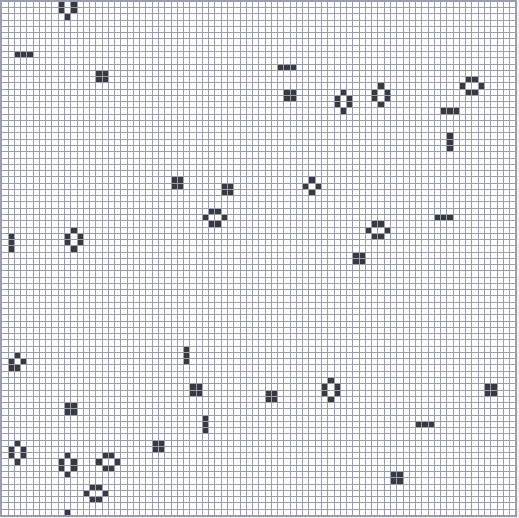
\includegraphics[width=5cm]{life.png}
\caption{Przykładowy stan automatu \textit{Life}. }
\label{fig:2figsA}}
\qquad
\begin{minipage}{7cm}
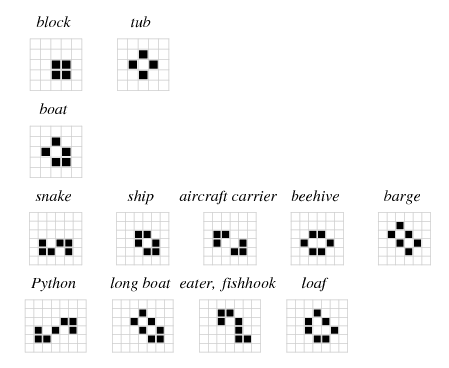
\includegraphics[width=7cm]{struktury.png}
\caption{Różne struktury powstające przy automacie \textit{Life}. Źródło \textit{mathworld.wolfram.com/GameofLife.html}}
\label{fig:2figsB}
\end{minipage}
\end{figure}

\subsection{Skupiska}
Inną ciekawą regułą jest 4567/345 (\textit{Assimialtion}). Podczas ewolucji tworzą się skupiska, które pochłaniają stopniowo całą siatkę (jeśli gęstość siatki jest powyżej ok. 16\%). Podobną regułą jest 5678/35678 (\textit{Diamoeba}), gdzie również tworzą się grupy, jednak są bardziej zwarte. Dla tego automatu początkowa gęstość siatki musi być odpowiednio wysoka - około 48\%, inaczej automat szybko osiągnie stan stacjonarny.

\begin{figure}[H]
\centering
\parbox{5cm}{
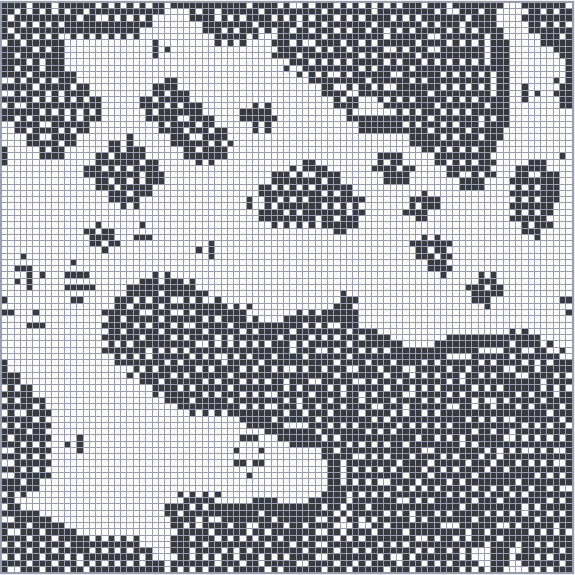
\includegraphics[width=5cm]{kolonie1.png}
\caption{Przykładowy stan automatu 4567/345. }
\label{fig:2figsA}}
\qquad
\begin{minipage}{5cm}
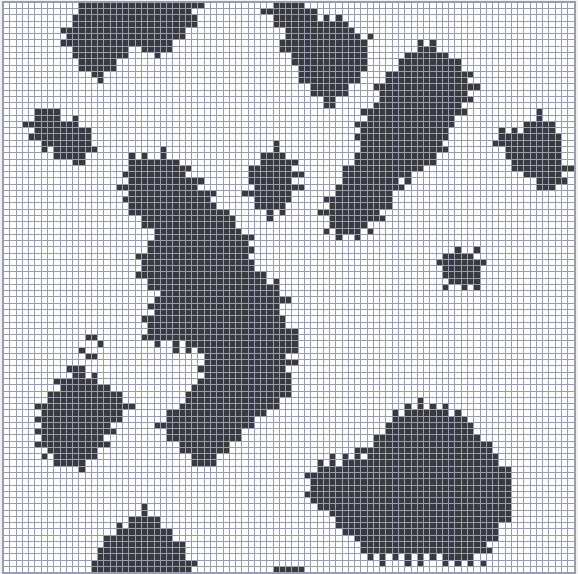
\includegraphics[width=5cm]{kolonie2.png}
\caption{Przykładowy stan automatu 5678/35678.}
\label{fig:2figsB}
\end{minipage}
\end{figure}

\subsection{Koralowiec}
Automat 45678/3 przypomina rozrastającego się koralowca. Choć początkowo komórki szybko wymierają, stopniowo ożywają, podobnie jak to żywe organizmy. Gdy automat posiada gęstość początkową powyżej 25\% i ustabilizuje się, większość komórek jest żywa i można zaobserwować sporadyczne pulsacje.

\subsection{Labirynt}
Stan końcowy automatu o regule 12345/3 (\textit{Maze}) przypomina labirynt z korytarzami. Z początkowego, chaotycznego stanu, szybko ewoluuje w określone wzory. Mogą wystąpić elementy oscylujące. Gęstość początkowa wystarczy aby była 3\%, a nawet 2\% przy szczęśliwym ułożeniu komórek.

\begin{figure}[H]
\centering
\parbox{5cm}{
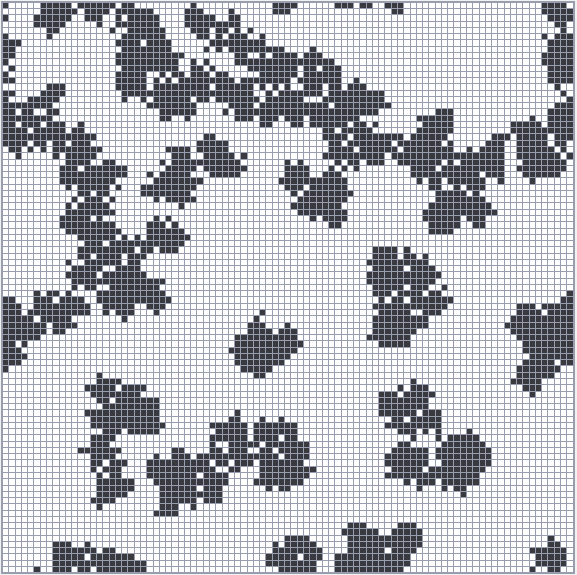
\includegraphics[width=5cm]{koralowiec.png}
\caption{Przykładowy stan automatu 45678/3.}
\label{fig:2figsA}}
\qquad
\begin{minipage}{5cm}
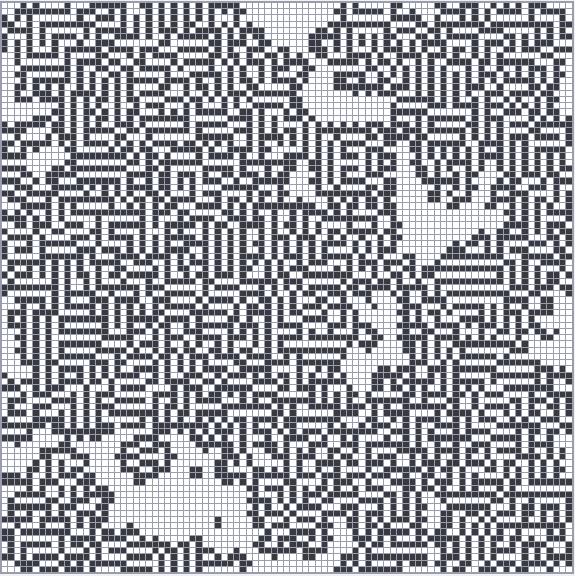
\includegraphics[width=5cm]{maze.png}
\caption{Przykładowy stan automatu 12345/3.}
\label{fig:2figsB}
\end{minipage}
\end{figure}

\section{Używanie aplikacji}
Użytkownik może dowolnie dobierać reguły, ustawiając parametry STAY i BORN. Możliwa jest również modyfikacja początkowej gęstości siatki oraz jej rozmiaru, za pomocą z menu ''Parametry wejściowe''. Poniżej menu znajduje się wykres prezentujący gęstość życia w symulacji dla kolejnych iteracji. Po prawej stronie aplikacji znajduje się siatka, na której prezentowane jest działanie automatu.

Symulacją można sterować za pomocą przycisków ''START'', ''RESET'' oraz ''STOP''. Gdy zostaną zmienione parametry, siatka jest automatycznie resetowana.

\begin{figure}[H]
\centering
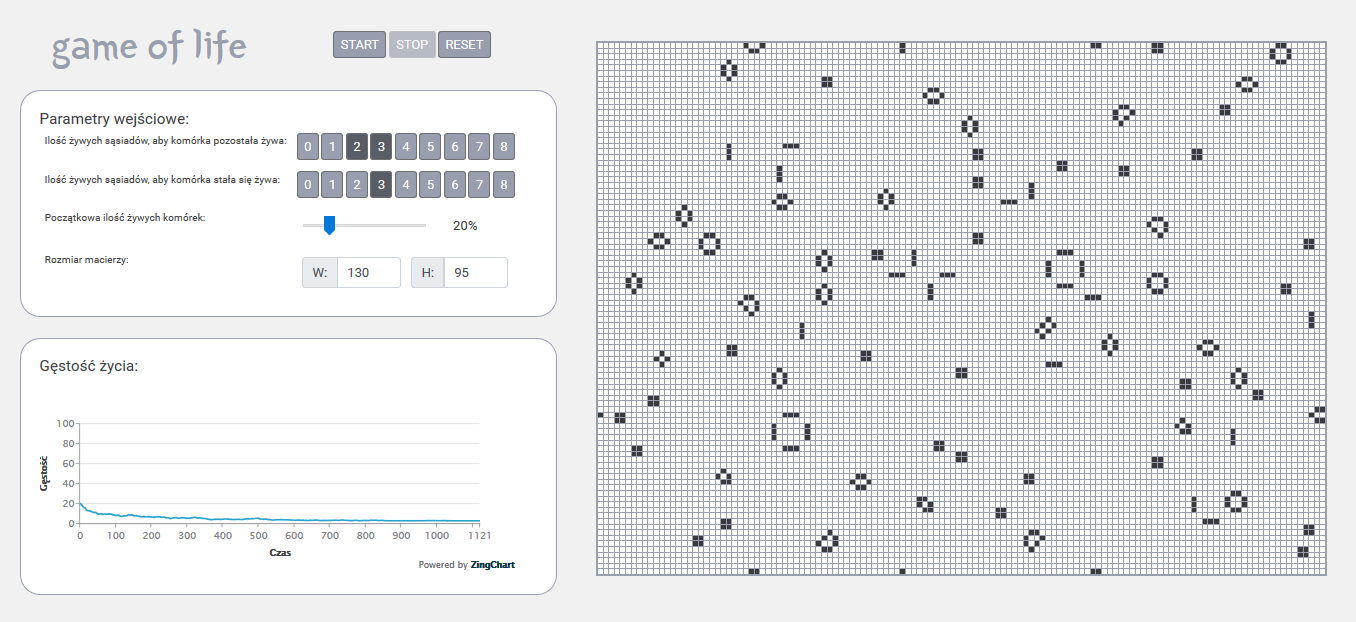
\includegraphics[width=14cm]{strona.png}
\caption{Widok aplikacji.}
\end{figure}

Do stworzenia strony zostały użyte technologie HTML + JS + CSS oraz ZingChart do rysowania wykresu.

\end{document}
